\section{梯度}

通过方向导数我们可以看到,若一个函数可微则任何方向的导数可以分解为两个偏导的线性组合,于是偏导可以认为是一个坐标系。
本节将这个概念定义化。

本节要点:
\begin{itemize}
    \item 掌握梯度的概念;
    \item 理解梯度的几何意义;
    \item 理解微分算子的概念。
\end{itemize}

%============================================================
\subsection{梯度的概念}

\begin{definition}[梯度]
设函数$z=z\left( \boldsymbol{p} \right) $在一点处可微,则称其两个偏导构成的矢量$\left( \frac{\partial z}{\partial x}\,\,\frac{\partial z}{\partial y} \right) ^T$为{\bf $z=z\left( \boldsymbol{p} \right) $在该点处的梯度},记为$\mathbf{grad}z$,简记为$\nabla z$,即:
\[
\nabla z:=\left( \begin{array}{c}
	\frac{\partial z}{\partial x}\\
	\frac{\partial z}{\partial y}\\
\end{array} \right)
\]
\end{definition}

梯度的特点:
\begin{itemize}
    \item 梯度是一个矢量,由对各个坐标的偏导构成;
    \item 梯度的方向就是最大的方向导数的方向;
    \item 梯度的模就是最大的方向导数的值。
\end{itemize}

于是,我们可以用梯度描述方向导数,如下:
\[
\frac{\partial z}{\partial n}=\frac{\partial z}{\partial x}\cos \alpha +\frac{\partial z}{\partial y}\cos \beta =\nabla z^T\mathbf{n}=\left\| \nabla z \right\| \cos \theta
\]
其中,
\begin{itemize}
    \item $\mathbf{n}=\left( \cos \alpha \,\,\cos \beta \right) ^T$:方向$n$的方向余弦;
    \item $\theta $:方向$n$和梯度的夹角。
\end{itemize}

\begin{figure}[h]
\centering
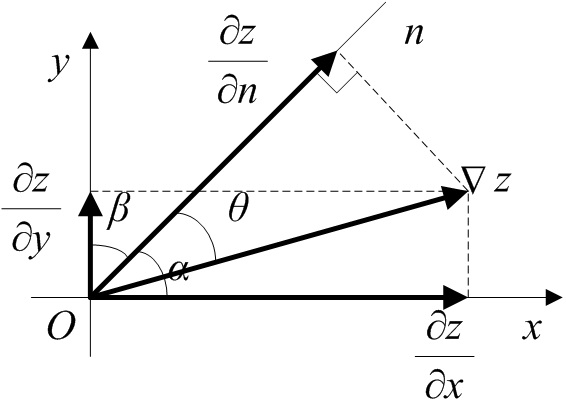
\includegraphics[height=3.5cm]{7.4.png}
\end{figure}

%============================================================
\subsection{梯度的几何意义}

几何上,梯度与等值线有垂直关系。
以二维平面的数量场为例,点$\boldsymbol{p}_0$的梯度:
\begin{itemize}
    \item 方向是等值线上该点的法向方向;
    \item 大小是$\left. \left\| \nabla z \right\| \right|_{\boldsymbol{p}_0}$。
\end{itemize}

\begin{figure}[h]
\centering
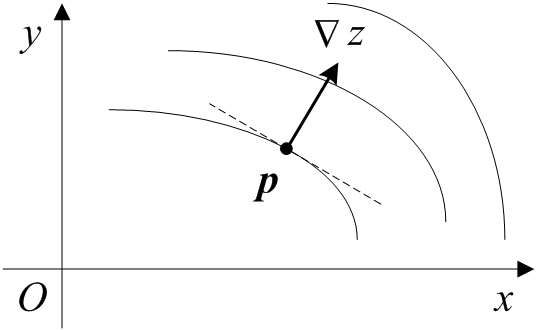
\includegraphics[height=3cm]{7.5.png}
\end{figure}

%============================================================
\subsection{梯度的物理意义}

物理上任何一个数量场,只要有变化(无变化也可以)都会有变化率,变化率可以分解到{\it xy}坐标,构成一个矢量。
所以,只有数量场才有梯度,是一个描述数量场的变化率的矢量场,其次梯度是由数量场决定的,可以认为是该数量场的性质。

%============================================================
\subsection{向量微分算子}

从纯粹的数学上,可以再进一步把“计算梯度”这一数学计算抽象出来,写成记号:
\[
\nabla :=\left( \begin{array}{c}
	\frac{\partial}{\partial x}\\
	\frac{\partial}{\partial y}\\
\end{array} \right)
\]
称为{\bf 向量微分算子},又称{\bf 哈密尔顿算子}:
\begin{itemize}
    \item 首先,它是一个算子,是纯数学上的一个计算符号,本身不承载任何物理意义;
    \item 其次是一个进行微分运算的算子;
    \item 最后是向量,表示这个微分算子是对构成其目标对象的基的微分运算,结果是一个矢量。
\end{itemize}
于是,梯度可以理解为微分算子和数量场的积,或者更简单的是“一个矢量的数乘”:
\[
\nabla z=\left( \begin{array}{c}
	\frac{\partial}{\partial x}\\
	\frac{\partial}{\partial y}\\
\end{array} \right) z=\left( \begin{array}{c}
	\frac{\partial z}{\partial x}\\
	\frac{\partial z}{\partial y}\\
\end{array} \right)
\]

~

梯度的运算法则:
\begin{align*}
&\nabla Cf=C\nabla f \\
&\nabla \left( f+g \right) =\nabla f+\nabla g \\
&\nabla \left( fg \right) =g\nabla f+f\nabla g \\
&\nabla f\left( u \right) =\frac{df}{du}\nabla u
\end{align*}




